\documentclass[UTF8,a4paper,12pt]{ctexart} 

\usepackage{graphicx}%学习插入图
\usepackage{verbatim}%学习注释多行
\usepackage{booktabs}%表格
\usepackage{geometry}%图片
\usepackage{amsmath}
\usepackage{amssymb}
\usepackage{listings}%代码
\usepackage{xcolor}  %颜色
\usepackage{enumitem}%列表格式
\setenumerate[1]{itemsep=0pt,partopsep=0pt,parsep=\parskip,topsep=5pt}
\setitemize[1]{itemsep=0pt,partopsep=0pt,parsep=\parskip,topsep=5pt}
\setdescription{itemsep=0pt,partopsep=0pt,parsep=\parskip,topsep=5pt}
\usepackage{tcolorbox}
\usepackage{algorithm}  %format of the algorithm
\usepackage{algorithmic}%format of the algorithm
\usepackage{multirow}   %multirow for format of table
\usepackage{tabularx} 	%表格排版格式控制
\usepackage{array}	%表格排版格式控制
\usepackage{hyperref} %超链接 \url{URL}
\usepackage{tikz}
\usepackage{dirtree}


\usetikzlibrary{intersections,
	positioning,
	petri,
	backgrounds,
	fit,
	decorations.pathmorphing,
	arrows,
	arrows.meta,
	bending,
	calc,
	intersections,
	through,
	backgrounds,
	shapes.geometric,
	quotes,
	matrix,
	trees,
	shapes.symbols,
	graphs,
	math,
	patterns,
	external}
\CTEXsetup[format+={\flushleft}]{section}

%%%% 设置图片目录
\graphicspath{{figure/}}

%%%% 段落首行缩进两个字 %%%%
\makeatletter
\let\@afterindentfalse\@afterindenttrue
\@afterindenttrue
\makeatother
\setlength{\parindent}{2em}  %中文缩进两个汉字位

%%%% 下面的命令重定义页面边距,使其符合中文刊物习惯 %%%%
\addtolength{\topmargin}{-54pt}
\setlength{\oddsidemargin}{0.63cm}  % 3.17cm - 1 inch
\setlength{\evensidemargin}{\oddsidemargin}
\setlength{\textwidth}{14.66cm}
\setlength{\textheight}{24.00cm}    % 24.62

%%%% 下面的命令设置行间距与段落间距 %%%%
\linespread{1.4}
\setlength{\parskip}{0.5\baselineskip}
\geometry{left=1.6cm,right=1.8cm,top=2cm,bottom=1.7cm} %设置文章宽度
\pagestyle{plain} 		  %设置页面布局

%代码效果定义
\definecolor{mygreen}{rgb}{0,0.6,0}
\definecolor{mygray}{rgb}{0.5,0.5,0.5}
\definecolor{mymauve}{rgb}{0.58,0,0.82}
\lstset{ %
	backgroundcolor=\color{white},   % choose the background color
	basicstyle=\footnotesize\ttfamily,      % size of fonts used for the code
	%stringstyle=\color{codepurple},
	%basicstyle=\footnotesize,
	%breakatwhitespace=false,         
	%breaklines=true,                 
	%captionpos=b,                    
	%keepspaces=true,                 
	%numbers=left,                    
	%numbersep=5pt,                  
	%showspaces=false,                
	%showstringspaces=false,
	%showtabs=false,        
	columns=fullflexible,
	breaklines=true,                 % automatic line breaking only at whitespace
	captionpos=b,                    % sets the caption-position to bottom
	tabsize=4,
	commentstyle=\color{mygreen},    % comment style
	escapeinside={\%*}{*)},          % if you want to add LaTeX within your code
	keywordstyle=\color{blue},       % keyword style
	stringstyle=\color{mymauve}\ttfamily,     % string literal style
	frame=single,
	rulesepcolor=\color{red!20!green!20!blue!20},
	% identifierstyle=\color{red},
	language=c++,
}
 \author{\kaishu 郑华}
 \title{\heiti Unity 优化基础}
 
\begin{document}          %正文排版开始
 	\maketitle
 	
 	\newpage
 	\tableofcontents
 	
  \newpage
  \section{基础}
	  	\paragraph{DrawCall}
	  		\verb|drawcall|是啥?其实\textbf{就是对底层图形程序}(比如:\verb|OpenGL ES|)\textbf{接口的调用},\textit{以在屏幕上画出东西}。
	  			
	  			\dirtree{%
	  				.1 \textbf{一个DrawCall} .
	  				.2 一次 DirectX -> DrawIndexedPrimitive() .
	  				.2 一次 OpenGL -> DrawElements() .
	  				.2 一个 Batch .
	  			}
	  		
	  		所以,是\textbf{谁去调用这些接口}呢?\verb|--> CPU|。
	  		
	  	\paragraph{Fragment}
	  		\verb|VF(Vertex,Fragment)|,\verb|Vertex|是\textbf{顶点},那\verb|Fragment|是啥呢?说它之前需要先说一下\textbf{像素},像素是构成\textbf{数码影像}的基本单元呀。e而\verb|Fragment|是有可能成
	  		为\textbf{像素}的东西。啥叫有可能?就是\textit{最终会不会被画出来不一定,是潜在的像素}。
	  		
	  		所以,这会\textbf{涉及到谁}呢?\verb|--> GPU|。
	  		
	  	\paragraph{Batching}
	  		\verb|batching|是啥?\textit{将}\textbf{批处理}\textit{之前需要很多次调用(drawcall)的物体}\textbf{合并},\textbf{之后只需要调用一次底层图形程序的接口就行}。听上去这简直就是优化的终极方案啊!但是,理想是美好的。
	  		
	  		\subparagraph{例子}
	  			如果在画面上有一张 “木" 椅子、一张 “铁" 桌子,既兩物件分别使用不同材质球或者不同的 Shader,那么理论上就会有两个 Draw Call。
	  			
	  			在 DirectX 或 OpenGL 里,对不同物件指定不同贴图或不同 Shader 的描述,就会需要呼叫兩次Draw Call。具体的伪代码如下:
	  				\begin{lstlisting}[frame = L, xleftmargin = .079\textwidth]
	 // 渲染桌子
	 SetShader( “Diffuse" );
	 SetTexture( “铁" );
	 DrawPrimitive( DeskVertexBuffer );   	
	 
	 // 渲染椅子
	 SetShader( “VertexLight" );
	 SetTexture( “木" );
	 DrawPrimitive( ChairVertexBuffer );				
	  				\end{lstlisting}
	  			
	  			每次对 Sahder 的变动或者贴图的变动,基本上就是对 Rendering Pipeline 的设定做修改,所以需要不同的 Draw Call 来完成物件的绘制。这就是为什么 UNITY 官方文件里,要你尽量使用相同的材质球,就是为了以減少 Draw Call 的数量!
	  			
	  			
	  			\verb|-->Notice: |而\verb|Batch| 就是把\underline{材质球相同的(Shader)}、\underline{贴图相同的(Texture)}、\textbf{用一个DrawCall 优化的手段}。
	  			
	  	\paragraph{内存的分配}
	 		除了\verb|Unity3D自己的内存|损耗。我们可是还带着Mono呢啊,还有\verb|托管的那一套|东西呢。更别说你一激动,又引入了\verb|自己的几个dll|。这些都是内存开销上需要考虑到的。
	 
	 
	 	\paragraph{总结}
	 		对于普通的优化需要注意的方面有以下三个方面:\verb|CPU |、\verb|GPU |、\verb|Memory |。
 		
  \section{CPU 方面的优化}
	  	\subsection{DrawCalls}
	  		\verb|DrawCall|是\textbf{CPU调用底层图形接口}。比如有上千个物体,每一个的渲染都需要去调用一次底层接口,而每一次的调用CPU都需要做很多工作,那么CPU必然不堪重负。但是对于GPU来说,图形处理的工作量是一样的。
	  		
	  		所以\textbf{对DrawCall的优化},\textit{主要}就是\textbf{为了尽量解放CPU在调用图形接口上的开销}。所以针对drawcall我们\textbf{主要的思路}就是\textit{每个物体尽量减少渲染次数},\textit{多个物体最好一起渲染}。所以,按照这个思路就有了以下几个方案:
	  			\begin{enumerate}
	  				\item 使用\verb|Draw Call Batching|,也就是\textbf{描绘调用批处理}。Unity在运行时可以将一些物体进行合并,从而用一个描绘调用来渲染他们。具体下面会介绍。
	  				\item 通过把\textbf{纹理打包成图集}来尽量减少材质的使用。
	  				\item \textbf{尽量少的使用反光},阴影之类的,因为那会使物体多次渲染。
	  			\end{enumerate}
	  	\subsection{Draw Call Batching}
	  		首先我们\textbf{要先理解}\textit{为何2个没有使用相同材质的物体即使使用批处理,也无法实现Draw Call数量的下降和性能上的提升}。
	  		
	  		\textbf{因为}被“批处理”的2个物体的网格模型需要使用相同材质的目的,在于其纹理是相同的,这样才可以实现同时渲染的目的。因而保证材质相同,是为了保证被渲染的纹理相同。
	  		
	  		\textbf{因此},为了将2个纹理不同的材质合二为一,我们就需要进行上面列出的第二步,\textbf{将纹理打包成图集}。\textit{具体到合二为一这种情况,就是将2个纹理合成一个纹理}。这样我们\textbf{就可以只用一个材质来代替之前的2个材质了}。
	  		
	  		而\verb|Draw Call Batching|本身,也还会\textbf{细分为2种}-静态批处理、动态批处理。
	  		
			  	\subsubsection*{Static Batching}
			  		\textbf{静态?那就是不动的咯}。还有呢?额,听上去状态也不会改变,没有“生命”,比如山山石石,楼房校舍啥的。那和什么比较类似呢?嗯,聪明的各位一定觉得和场景的属性很像吧!所以我们的场景似乎就可以采用这种方式来减少draw call了。
			  		
			  		那么写个定义:\textbf{只要这些物体不移动,并且拥有相同的材质,静态批处理就允许引擎对任意大小的几何物体进行批处理操作来降低描绘调用。}
			  		
			  		那要如何使用静态批来减少Draw Call呢?你只需要明确指出哪些物体是静止的,并且在游戏中永远不会移动、旋转和缩放。想完成这一步,你只需要在检测器(Inspector)中将Static复选框打勾即可,如下图所示:
			  			\begin{figure}[H]
			  				\centering
			  				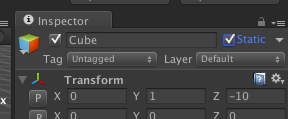
\includegraphics[scale=1]{beforeStaticBatching.png}
			  				\caption{设置}
			  			\end{figure}
		  			
		  			至于效果如何呢?
		  			
		  			举个例子:新建4个物体,分别是\verb|Cube|,\verb|Sphere|, \verb|Capsule|, \verb|Cylinder|,它们有\textbf{不同的网格模型},但是也\verb|有相同的材质(Default-Diffuse)|。
		  			
		  			\textbf{首先},我们\textit{不指定它们是static的}。\textbf{Draw Call的次数是4次},如图:
		  				\begin{figure}[H]
		  					\centering
		  					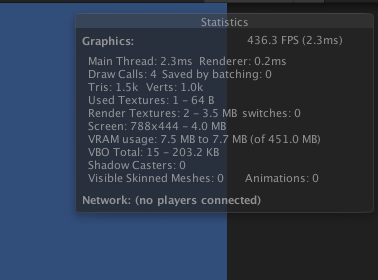
\includegraphics[scale=0.8]{beforeStaticBatching2.png}
		  					\caption{未设置静态批处理}
		  				\end{figure}
		  			
		  			我们\textbf{现在将它们4个物体都设为static},在来运行一下:
		  				\begin{figure}[H]
		  					\centering
		  					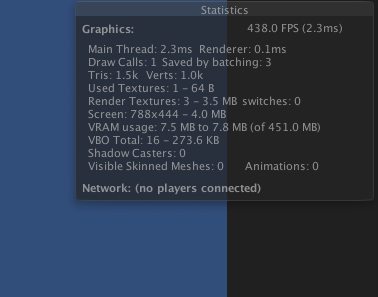
\includegraphics[scale=0.8]{afterStaticBatching.png}
		  					\caption{设置静态批处理后}
		  				\end{figure}
	  				
	  				如图,\textbf{Draw Call的次数变成了1},而\verb|Saved by batching|的次数变成了\verb|3|。
	  				
	  				\textbf{静态批处理}的好处很多,\textbf{其中之一}\textit{就是与下面要说的动态批处理相比,约束要少很多}。\textbf{所以一般推荐的是draw call的静态批处理来减少draw call的次数}。那么接下来,我们就继续聊聊draw call的动态批处理。
	  				
			  	\subsubsection*{Dynamic Batching}
	  				首先要明确一点,Unity3D的\textbf{draw call动态批处理机制}是\textit{引擎自动进行的},\textit{无需像静态批处理那样手动设置static}。我们举一个\verb|动态实例化prefab|的例子,如果动态物体\textbf{共享相同的材质},\textit{则引擎会自动对draw call优化,也就是使用批处理}。首先,我们将一个\verb|cube|做成\verb|prefab|,然后再实例化500次,看看\verb|draw call|的数量。
	  				
	  				\begin{lstlisting}[frame=L, xleftmargin = .079\textwidth]
	for(int i = 0; i < 500; i++)
	{
		GameObject cube;
		cube = GameObject.Instantiate(prefab) as GameObject;
	}
	  				\end{lstlisting}
	  				
	  				\verb|draw call|的数量:
	  				\begin{figure}[H]
	  					\centering
	  					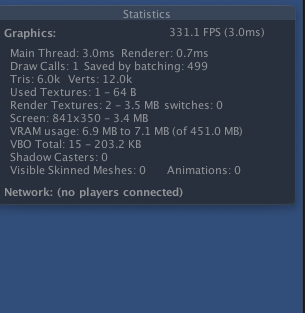
\includegraphics[scale=0.8]{afterDynamicBatching2.png}
	  					\caption{动态批处理-1}
	  				\end{figure}
	  				
	  				
	  				可以看到\verb|draw call|的数量为1,而 \verb|saved by batching|的数量是499。而这个过程中,我们除了实例化创建物体之外什么都没做。不错,unity3d引擎为我们自动处理了这种情况。
	  				
	  				但是有很多童靴也遇到\textbf{这种情况},就是我也是\textbf{从prefab实例化创建的物体,为何我的draw call依然很高呢}?这就是匹夫上文说的,\verb|draw call|的\textbf{动态批处理存在着很多约束}。
	  				
	  				下面就演示一下,\textbf{针对cube这样一个简单的物体的创建,如果稍有不慎就会造成draw call飞涨的情况}。
	  				
	  				我们同样是创建500个物体,\textbf{不同的}是\textit{其中的100个物体},每个物体的\textit{大小都不同},也就是\textit{Scale不同}。
	  				\begin{lstlisting}[frame=L, xleftmargin = .079\textwidth]
	for(int i = 0; i < 500; i++)
	{
		GameObject cube;
		cube = GameObject.Instantiate(prefab) as GameObject;
		if(i / 100 == 0)
		{
			cube.transform.localScale = new Vector3(2 + i, 2 + i, 2 + i);
		}
	}
	  				\end{lstlisting}
	  				\begin{figure}[H]
	  					\centering
	  					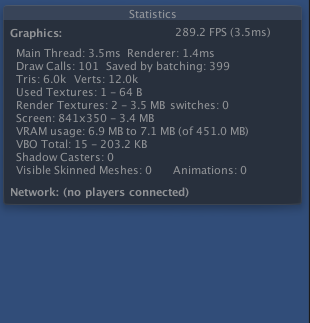
\includegraphics[scale=0.8]{afterDynamicBatching.png}
	  					\caption{动态批处理-2}
	  				\end{figure}
  				
  				我们看到\verb|draw call|的数量\textbf{上升到了101次},而\verb|saved by batching|的数量也下降到了399。各位看官可以看到,仅仅是一个简单的\verb|cube|的创建,如果\verb|scale|不同,竟然也不会去做批处理优化。
  				
  				\textbf{这仅仅是动态批处理机制的一种约束},那我们\textbf{总结一下动态批处理的约束},各位也许也能从中找到为何动态批处理在自己的项目中不起作用的原因:
  					\begin{enumerate}
		  				\item 批处理动态物体需要在每个顶点上进行一定的开销,所以\textbf{动态批处理仅支持小于900顶点的网格物体}。
		  				\item \textbf{如果}你的\textbf{着色器}使用\textbf{顶点位置,法线和UV值}\textit{三种属性},\textbf{那么你只能批处理300顶点以下的物体};\textbf{如果}你的\textbf{着色器}需要使用\textit{顶点位置,法线,UV0,UV1和切向量},那你只能批处理180顶点以下的物体。
		  				\item \textbf{不要使用缩放}。分别拥有缩放大小(1,1,1) 和(2,2,2)的两个物体\textbf{将不会进行批处理}。
		  				\item 统一缩放的物体不会与非统一缩放的物体进行批处理。
		  				\item 使用缩放尺度(1,1,1) 和 (1,2,1)的两个物体将不会进行批处理,但是使用缩放尺度(1,2,1) 和(1,3,1)的两个物体将可以进行批处理。
		  				\item \textbf{使用不同材质的实例化物体(instance)将会导致批处理失败}。
		  				\item 拥有lightmap的物体含有额外(隐藏)的材质属性,比如:lightmap的偏移和缩放系数等。所以,\textbf{拥有lightmap的物体将不会进行批处理}(\textit{除非他们指向lightmap的同一部分})。
		  				\item \textbf{多通道的shader会妨碍批处理操作}。比如,几乎unity中所有的着色器在前向渲染中都支持多个光源,并为它们有效地开辟多个通道。
		  				\item \textbf{预设体的实例会自动地使用相同的网格模型和材质}。
	  				\end{enumerate}
	  			
	  			所以,\textbf{尽量使用静态的批处理}。
	  			
	  	\subsection{物理组件}
	  		从性能优化的角度考虑,物理组件能少用还是少用为好。
	  		
	  	\subsection{处理内存-GC}
	  		虽然GC是用来处理内存的,但的确增加的是CPU的开销。因此它的确能达到释放内存的效果,但代价更加沉重,会加重CPU的负担,因此\textbf{对于GC的优化目标}就是\textit{尽量少的触发GC}。
	  		
	  		\textbf{首先}我们要明确所谓的\textbf{GC是Mono运行时的机制},\textit{而非Unity3D游戏引擎的机制},所以\textbf{GC也主要是针对Mono的对象来说的},\textbf{而它管理的也是Mono的托管堆}。
	  		
	  		搞清楚这一点,你也就明白了\verb|GC |\textbf{不是用来处理引擎的}\textit{ assets(纹理啦,音效啦等等)的内存释放}的,\textbf{因为U3D引擎也有自己的内存堆而不是和Mono一起使用所谓的托管堆}。
	  		
	  		\textbf{其次}我们要搞清楚\textbf{什么东西会被分配到托管堆上}?是\textbf{引用类型}。比如\textbf{类的实例},\textbf{字符串},\textbf{数组}等等。\textit{而作为int,float,包括结构体struct其实都是值类型,它们会被分配在栈上而非堆上}。所以\textbf{我们关注的对象无外乎就是类实例,字符串,数组这些了}。
	  		
	  		那么\textbf{GC什么时候会触发}呢?两种情况:
	  			\begin{enumerate}[itemindent = 2em]
	  				\item 首先\textbf{堆的内存不足时},会自动调用GC。
	  				\item 其次也可以通过编程\textbf{手动的调用}GC。
	  			\end{enumerate}
	  		
	  		
	  		\textbf{所以为了达到优化CPU的目的,我们就不能频繁的触发GC。}而上文也说了GC处理的是托管堆,而不是Unity3D引擎的那些资源,\textbf{所以GC的优化说白了也就是代码的优化。}那么匹夫觉得有以下几点是需要注意的:
	  			\begin{enumerate}[itemindent = 2em]
	  				\item \textbf{字符串连接的处理。}\textit{因为将两个字符串连接的过程,其实是生成一个新的字符串的过程。而之前的旧的字符串自然而然就成为了垃圾。而作为引用类型的字符串,其空间是在堆上分配的,被弃置的旧的字符串的空间会被GC当做垃圾回收。}
	  				\item \textbf{尽量不要使用foreach,而是使用for}。\textit{foreach其实会涉及到迭代器的使用,而据传说每一次循环所产生的迭代器会带来24 Bytes的垃圾。那么循环10次就是240Bytes。}
	  				\item \textbf{不要直接访问gameobject的tag属性}。比如\verb|if(go.tag == “human”)|最好换成\verb|if(go.CompareTag (“human”))|。\textit{因为访问物体的tag属性会在堆上额外的分配空间。}如果在循环中这么处理,留下的垃圾就可想而知了。
	  				\item \textbf{使用“池”,以实现空间的重复利用}。
	  			\end{enumerate}
	  		
	  		
	  	\subsection{代码-脚本}
  			这里要提到的所谓代码质量是基于一个前提的:Unity3D是用C++写的,而我们的代码是用C\#作为脚本来写的,那么问题就来了~\textbf{脚本和底层的交互开销是否需要考虑呢?}也就是说,\textbf{我们用Unity3D写游戏的“游戏脚本语言”,也就是C\#是由mono运行时托管的}。而功能是底层引擎的C++实现的,\textbf{“游戏脚本”中的功能实现都离不开对底层代码的调用。那么这部分的开销,我们应该如何优化呢}?
  			
  			\paragraph{调用方式}\verb|->|
  			
	  			以物体的\verb|Transform组件|为例,我们应该只访问一次,之后就将它的引用保留,而非每次使用都去访问。这里有人做过一个小实验,就是对比通过方法\verb|GetComponent<Transform>()|获取\verb|Transform|组件, 通过\verb|MonoBehaviour的transform|属性去取,以及保留引用之后再去访问所需要的时间:
	  				\begin{itemize}
	  					\item \verb|GetComponent<Transform>()| = 619ms
	  					\item \verb|Monobehaviour.Tramsform| = 60ms
	  					\item \verb|CachedMB| = 8ms
	  					\item \verb|Manual Cache| = 3ms
	  				\end{itemize}
	  			
  				如上所述,\textbf{最好不要频繁使用}\verb|GetComponent|,尤其是在循环中。
  			
  			\paragraph{没用关闭可见性}\verb|->|
  			
  				善于使用\verb|OnBecameVisible()|,来控制物体的\verb|update()|函数的执行\textbf{以减少开销}。
  			
  			\paragraph{使用内建的数组}\verb|->|
  			
  				比如用\verb|Vector3.zero|而不是\verb|new Vector(0, 0, 0);|
  			
  			\paragraph{对于方法的参数的优化}\verb|->|
  			
  				善于使用\textbf{ref关键字}\verb|-->对象的传递都是引用|。
  				
  				值类型的参数,\textit{是通过将实参的值复制到形参,来实现按值传递到方法,也就是我们通常说的按值传递}。复制嘛,总会让人感觉很笨重。比如\verb|Matrix4x4|这样比较复杂的值类型,如果直接复制一份新的,反而不如将值类型的引用传递给方法作为参数。
  	
  \section{GPU 方面的优化}
  		GPU与CPU不同,所以\textbf{侧重点也不一样}。\textbf{GPU的瓶颈}主要存在\textbf{在如下的方面}:
  			\begin{itemize}
  				\item \textbf{填充率},可以简单的理解为\textit{图形处理单元每秒渲染的像素数量}。
  				\item \textbf{像素的复杂度},比如\textit{动态阴影,光照,复杂的shader}等等
  				\item \textbf{几何体的复杂度}(\textit{顶点数量})
  				\item \textbf{GPU的显存带宽}
  			\end{itemize}

  		那么针对以上4点,其实仔细分析我们就可以发现,影响的GPU性能的无非就是2大方面,\textbf{一方面是顶点数量过多,像素计算过于复杂}。\textit{另一方面就是GPU的显存带宽}。那么针锋相对的两方面举措也就十分明显了。
  			\begin{itemize}
  				\item 减少顶点数量,简化计算复杂度。
  				\item 压缩图片,以适应显存带宽。
  			\end{itemize}
  		
  		\subsection{减少绘制的数目}
  			那么第一个方面的优化也就是减少顶点数量,简化复杂度,具体的举措就总结如下了:
  			
  			\begin{itemize}
  				\item \textbf{保持材质的数目尽可能少}。这使得Unity更容易进行批处理。
  				\item \textbf{使用纹理图集}(一张大贴图里包含了很多子贴图)来代替一系列单独的小贴图。它们可以更快地被加载,具有很少的状态转换,而且批处理更友好。
  				\item \textbf{如果使用了纹理图集和共享材质,使用Renderer.sharedMaterial 来代替Renderer.material} 。
  				\item \textbf{使用光照纹理(lightmap)而非实时灯光}。
  				\item 使用LOD,好处就是对那些离得远,看不清的物体的细节可以忽略。
  				\item \textbf{遮挡剔除}(Occlusion culling)
  				\item 使用mobile版的shader。因为简单。
  			\end{itemize}
  			
  		\subsection{优化显存带宽}
  			第二个方向呢?压缩图片,减小显存带宽的压力。
  				\begin{itemize}
  					\item OpenGL ES 2.0使用ETC1格式压缩等等,在打包设置那里都有。
  					\item \textbf{使用mipmap}。
  				\end{itemize}
  			
  		\subsection{MipMap}
  			这里匹夫要着重介绍一下\verb|MipMap|到底是啥。因为有人说过\verb|MipMap|会占用内存呀,但为何又会优化显存带宽呢?那就不得不从\verb|MipMap|是什么开始聊起。一张图其实就能解决这个疑问。
  				\begin{figure}[H]
  					\centering
  					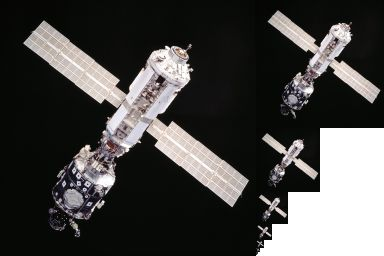
\includegraphics[scale=0.8]{mipMap.jpg}
  					\caption{上面是一个mipmap 如何储存的例子,左边的主图伴有一系列逐层缩小的备份小图}
  				\end{figure}
  			
  			是不是很一目了然呢?\verb|Mipmap|中每一个层级的小图都是主图的一个特定比例的缩小细节的复制品。因为存了主图和它的那些缩小的复制品,所以内存占用会比之前大。但是为何又优化了显存带宽呢?\textbf{因为可以根据实际情况,选择适合的小图来渲染。}所以,\textbf{虽然会消耗一些内存,但是为了图片渲染的质量(比压缩要好),这种方式也是推荐的}。
  			
  \section{内存方面的优化}
  		既然要聊Unity3D运行时候的内存优化,那我们自然首先要知道Unity3D游戏引擎是如何分配内存的。大概可以分成三大部分:
  			\begin{itemize}
  				\item Unity3D内部的内存
  				\item Mono的托管内存
  				\item 若干我们自己引入的DLL或者第三方DLL所需要的内存。
  			\end{itemize}
  		
  		\subsection{U3D 内部内存}
  			Unity3D的内部内存都会存放一些什么呢?各位想一想,除了用代码来驱动逻辑,一个游戏还需要什么呢?对,各种资源。所以简单总结一下Unity3D内部内存存放的东西吧:
  			\begin{itemize}
  				\item \verb|资源:纹理、网格、音频等等|
  				\item \verb|GameObject和各种组件。|
  				\item \verb|引擎内部逻辑需要的内存:渲染器,物理系统,粒子系统等等|
  			\end{itemize}
  			
  		\subsection{Mono托管内存}
  			因为我们的游戏脚本是用\verb|C#|写的,\textbf{同时还要跨平台},所以带着一个\textbf{Mono的托管环境}显然\textbf{必须的}。那么Mono的托管内存自然就不得不放到内存的优化范畴中进行考虑。那么我们所说的Mono托管内存中存放的东西和Unity3D内部内存中存放的东西究竟有何不同呢?其实Mono的内存分配就是很传统的运行时内存的分配了:
  			
  			\textbf{值类型}:\textit{int型啦,float型啦,结构体struct啦,bool啦之类的。它们都存放在堆栈上}(注意额,不是堆所以不涉及GC)。
  			
  			\textbf{引用类型}:\textit{其实可以狭义的理解为各种类的实例。}比如游戏脚本中对游戏引擎各种控件的封装。其实很好理解,\verb|C#|中肯定要有对应的类去对应游戏引擎中的控件。那么这部分就是\verb|C#|中的封装。由于是在堆上分配,所以会涉及到GC。
  			
  			\textbf{而Mono托管堆中的那些封装的对象,除了在在Mono托管堆上分配封装\underline{类实例化之后}所需要的内存之外,\underline{还会牵扯到其背后对应的游戏引擎内部控件在Unity3D内部内存上的分配}。}
  			
  			\subparagraph{例子-WWW}\verb|->|
  			
  				一个在\verb|.cs|\textbf{脚本中}声明的\textbf{WWW类型的对象www},\textit{Mono}会在\textbf{Mono托管堆}上\textbf{为www}分配它所需要的\textbf{内存}。同时,\underline{这个实例对象背后的所代表的引擎资源所需要的内存也需要被分配}。
  				
  				一个\verb|WWW|实例背后的资源:
  					\begin{itemize}
  						\item 压缩的文件
  						\item 解压缩所需的缓存
  						\item 解压缩之后的文件
  					\end{itemize}
  				
  				如下图所示:
  					\begin{figure}[H]
  						\centering
  						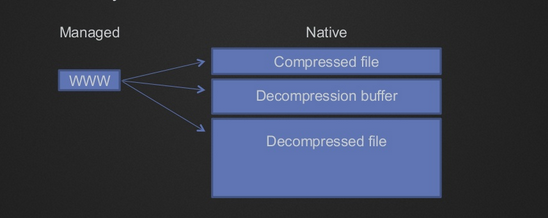
\includegraphics[scale=0.69]{Mono.png}
  						\caption{Mono 托管堆}
  					\end{figure}
  			
  			\subparagraph{例子-AssetBundle 内存处理}\verb|->|
  			
  				以下载Assetbundle为例子,聊一下内存的分配。
					\begin{lstlisting}
	IEnumerator DownloadAndCache ()
	{
		// Wait for the Caching system to be ready
		while (!Caching.ready)
			yield return null;
		
		// Load the AssetBundle file from Cache if it exists with the same version or download and store it in the cache
		using(WWW www = WWW.LoadFromCacheOrDownload (BundleURL, version))
		{
			yield return www; //WWW是第1部分
			if (www.error != null)
				throw new Exception("WWW download had an error:" + www.error);
			AssetBundle bundle = www.assetBundle;//AssetBundle是第2部分
			if (AssetName == "")
				Instantiate(bundle.mainAsset);//实例化是第3部分
			else
				Instantiate(bundle.Load(AssetName));
			// Unload the AssetBundles compressed contents to conserve memory
			bundle.Unload(false);
			
		} // memory is freed from the web stream (www.Dispose() gets called implicitly)
	}
					\end{lstlisting}
  		
  			内存分配的三个部分匹夫已经在代码中标识了出来:
  				\begin{itemize}
  					\item \verb|Web Stream|:包括了压缩的文件,解压所需的缓存,以及解压后的文件。
  					\item \verb|AssetBundle|:Web Stream中的文件的映射,或者说引用。
  					\item \verb|实例化之后的对象|:就是引擎的各种资源文件了,会在内存中创建出来。
  				\end{itemize}
  			
  			\begin{lstlisting}
  	WWW www = WWW.LoadFromCacheOrDownload (BundleURL, version)			
  			\end{lstlisting}
  			\begin{enumerate}
  				\item 将压缩的文件读入内存中
  				\item 创建解压所需的缓存
  				\item 将文件解压,解压后的文件进入内存
  				\item 关闭掉为解压创建的缓存
  			\end{enumerate}
  			
  			\begin{lstlisting}
  	AssetBundle bundle = www.assetBundle;		
  			\end{lstlisting}
  			\begin{enumerate}
  				\item AssetBundle此时相当于一个桥梁,从Web Stream解压后的文件到最后实例化创建的对象之间的桥梁。
  				\item 所以AssetBundle实质上是Web Stream解压后的文件中各个对象的映射。而非真实的对象。
  				\item 实际的资源还存在Web Stream中,所以此时要保留Web Stream。
  			\end{enumerate}
  			\begin{lstlisting}
  	Instantiate(bundle.mainAsset);		
  			\end{lstlisting}
  			通过AssetBundle获取资源,实例化对象。
  			最后各位可能看到了官网中的这个例子使用了:
  			
  			\verb|using(WWW www = WWW.LoadFromCacheOrDownload (BundleURL, version)){ }|

  			这种\verb|using|的用法。这种用法其实就是为了在使用完\verb|Web Stream|之后,将内存释放掉的。因为WWW也继承了\verb|idispose|的接口,所以可以使用\verb|using|的这种用法。其实相当于最后执行了:
  			\begin{lstlisting}
  	www.Dispose();	
  			\end{lstlisting}
  			OK,\verb|Web Stream|被删除掉了。那还有谁呢?对Assetbundle。那么使用
  			\begin{lstlisting}
  	bundle.Unload(false);		
  			\end{lstlisting}
  			
  		\subsection{使用 Unity Profier 检测内存}
  
	\section{参考}
		优化基础:\url{https://blog.csdn.net/cordova/article/details/52241249}
		
		相关解释:\url{https://blog.csdn.net/hany3000/article/details/44033243}	    
\end{document} 
 		    